% anhang.tex
% Weitere Informationen zum Projekt und zur Arbeit

\chapter{Auswertungen OLSR}
\label{appendix:olsr}

\begin{center}
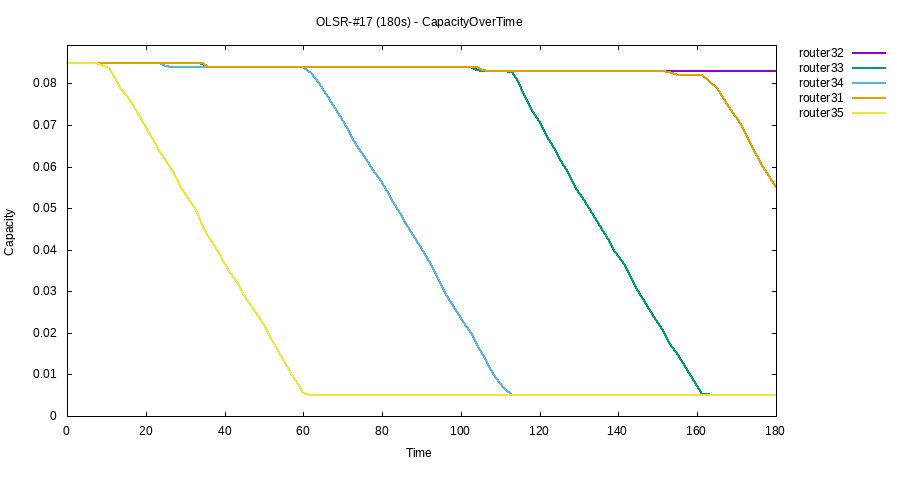
\includegraphics[scale=0.45]{bilder/os1.png} \\
\captionof{figure}{Verlauf Ladezustand bei OLSR, 180 Sekunden}
\end{center}

\begin{center}
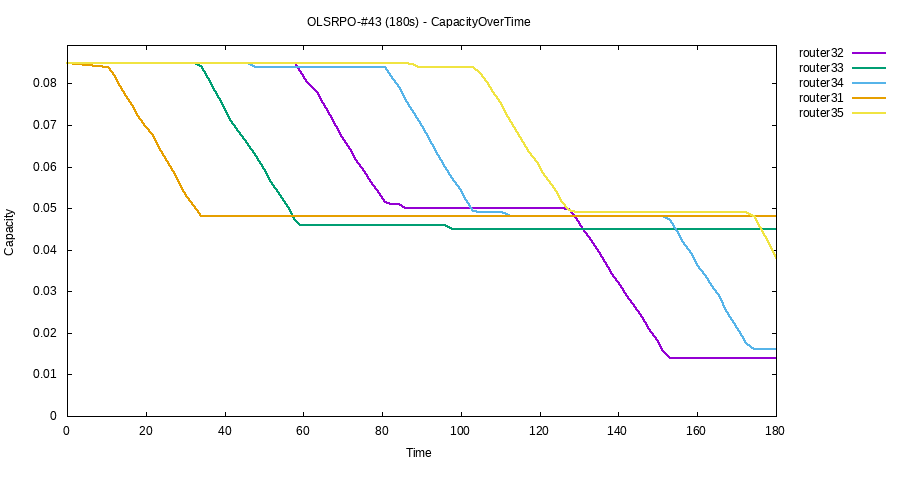
\includegraphics[scale=0.45]{bilder/os2.png} \\
\captionof{figure}{Verlauf Ladezustand bei OLSR-PO, 180 Sekunden}
\end{center}

\newpage

\begin{center}
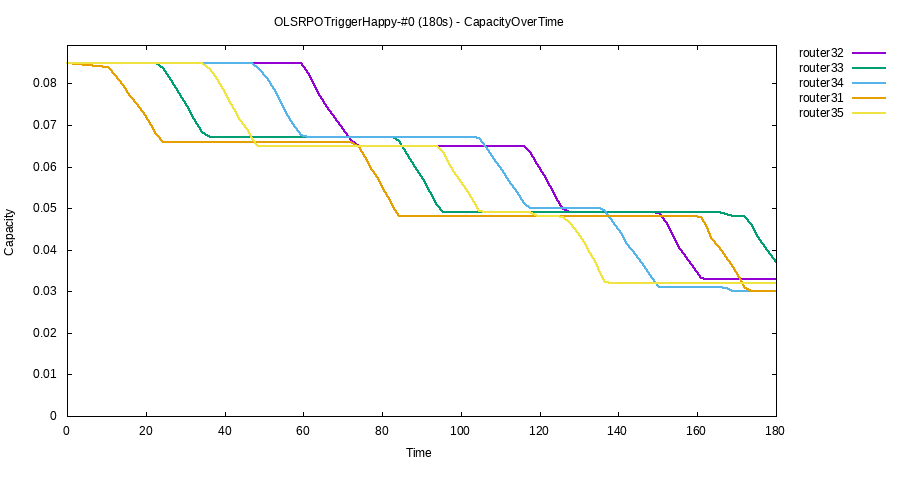
\includegraphics[scale=0.45]{bilder/os3.png} \\
\captionof{figure}{Niedrigerer Trigger $t=0.2$ bei OLSR-PO, 180 Sekunden}
\end{center}

\begin{center}
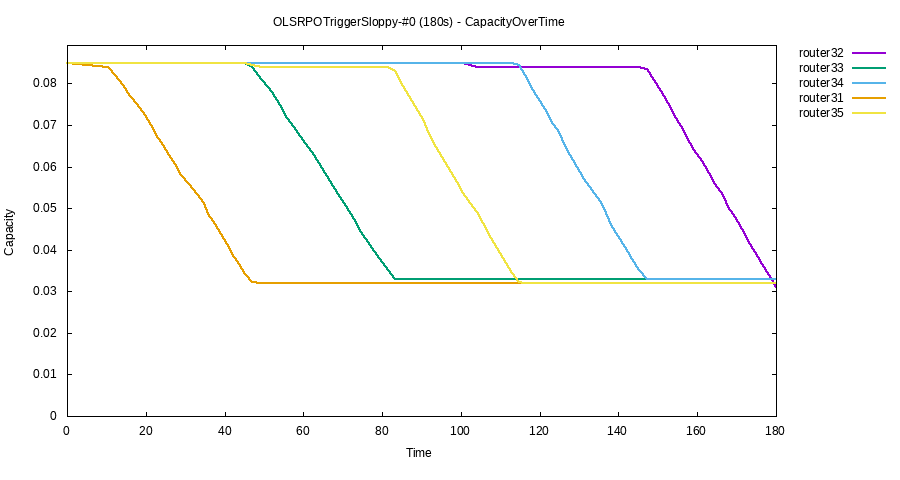
\includegraphics[scale=0.45]{bilder/os4.png} \\
\captionof{figure}{Höherer Trigger $t=0.4$ bei OLSR-PO, 180 Sekunden}
\end{center}

\begin{center}
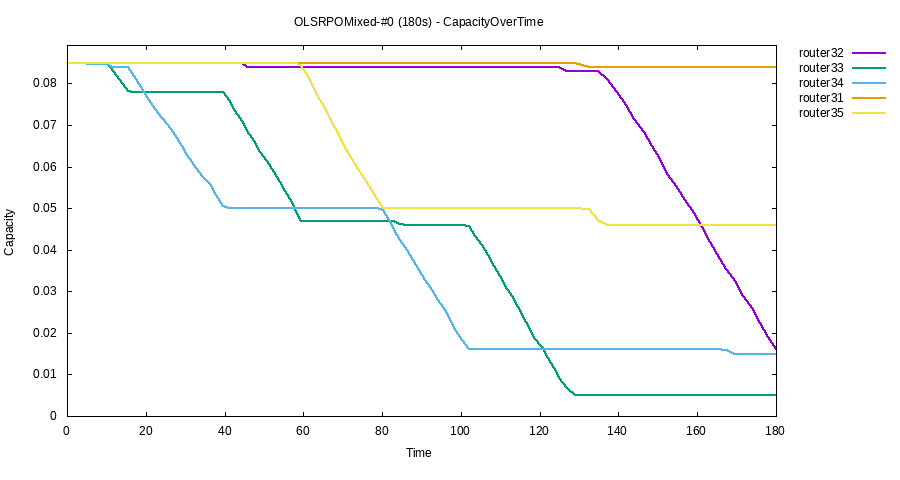
\includegraphics[scale=0.45]{bilder/os5.png} \\
\captionof{figure}{OLSR und OLSR-PO im Mischbetrieb, 180 Sekunden}
\end{center}


\chapter{Multi Hop}
\label{appendix:multihop}

\begin{center}
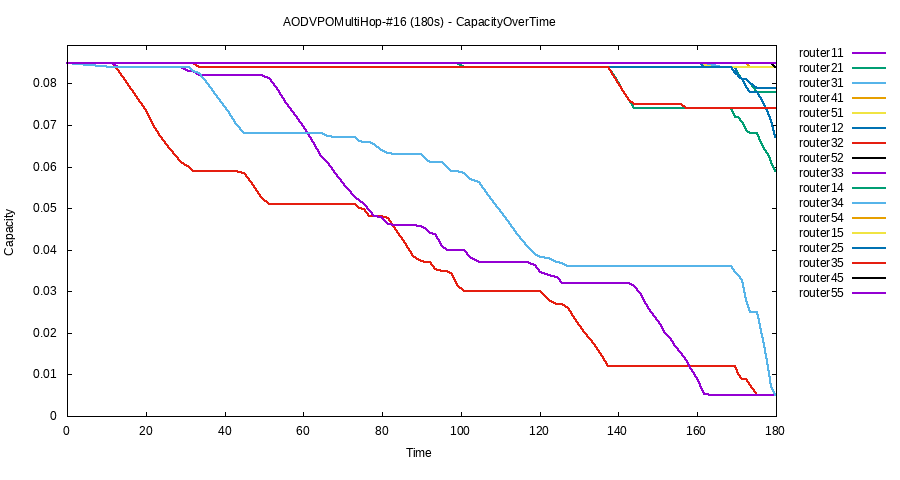
\includegraphics[scale=0.45]{bilder/m2.png} \\
\captionof{figure}{Verlauf Ladezustand bei AODV-PO im MutiHop Netz, 180 Sekunden}
\end{center}

\begin{center}
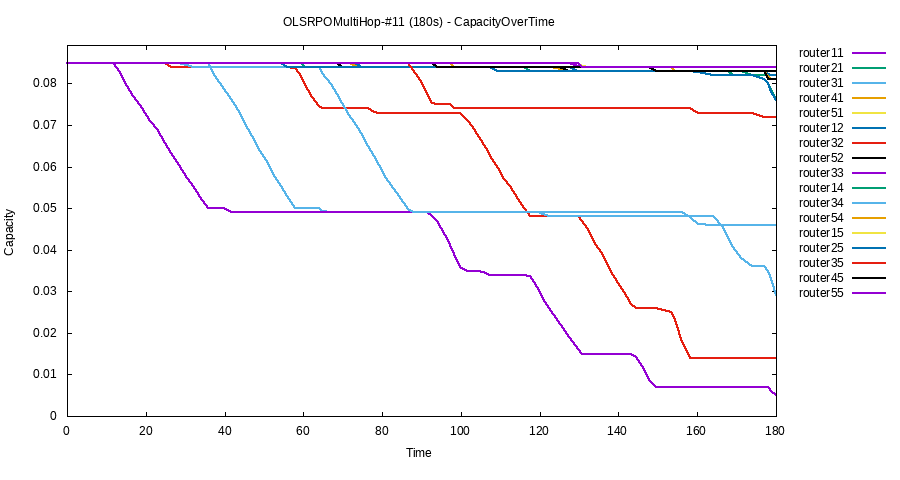
\includegraphics[scale=0.45]{bilder/m1.png} \\
\captionof{figure}{Verlauf Ladezustand bei OLSR-PO im MutiHop Netz, 180 Sekunden}
\end{center}

\chapter{Wiederholungen}
\label{appendix:repeat}

\begin{center}
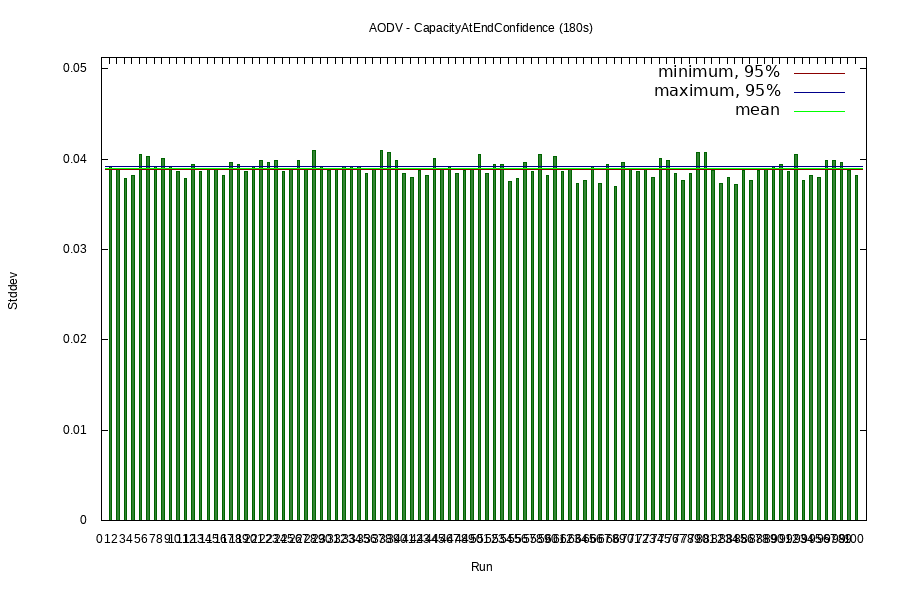
\includegraphics[scale=0.45]{bilder/sa4.png} \\
\captionof{figure}{Analyse Durchläufe AODV, 180 Sekunden}
\end{center}

\begin{center}
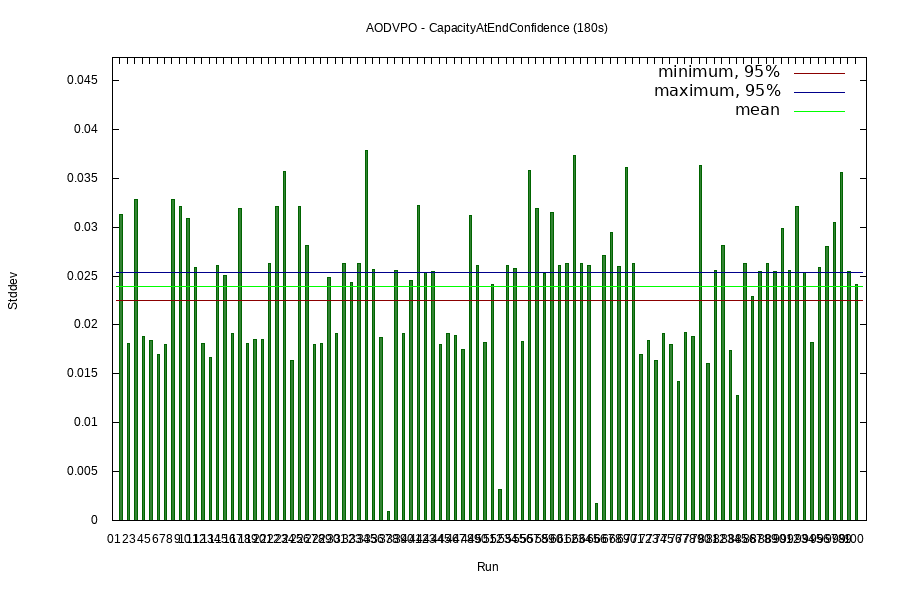
\includegraphics[scale=0.45]{bilder/sa5.png} \\
\captionof{figure}{Analyse Durchläufe AODV-PO, 180 Sekunden}
\end{center}

\newpage

\begin{center}
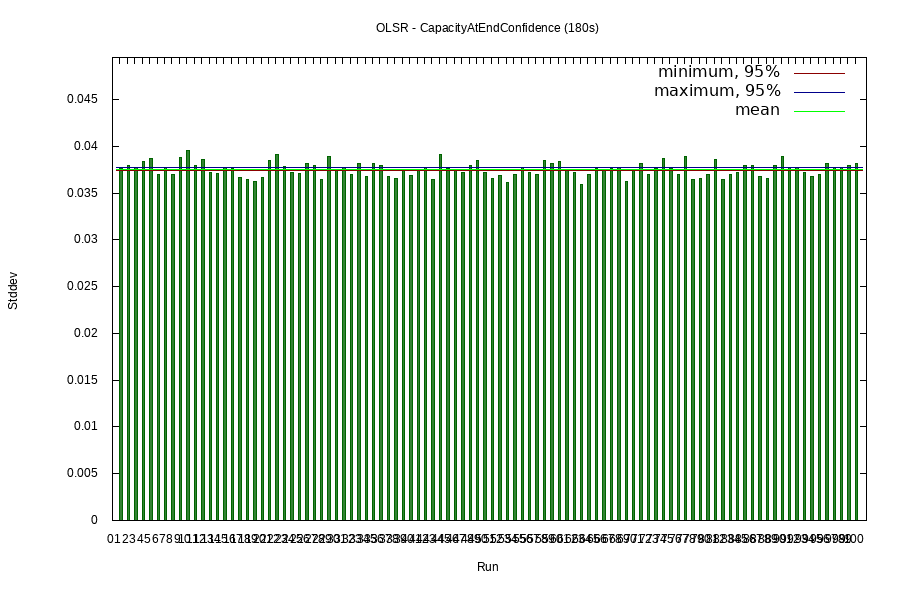
\includegraphics[scale=0.45]{bilder/so4.png} \\
\captionof{figure}{Analyse Durchläufe OLSR, 180 Sekunden}
\end{center}

\begin{center}
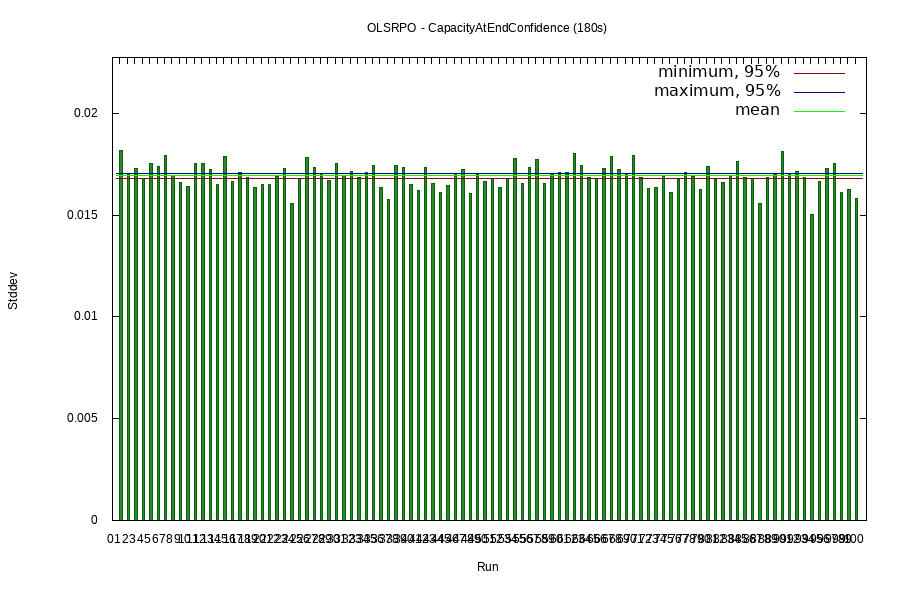
\includegraphics[scale=0.45]{bilder/so5.png} \\
\captionof{figure}{Analyse Durchläufe OLSR-PO, 180 Sekunden}
\end{center}

\chapter{3D Diagramme}
\label{appendix:3d}

\begin{center}
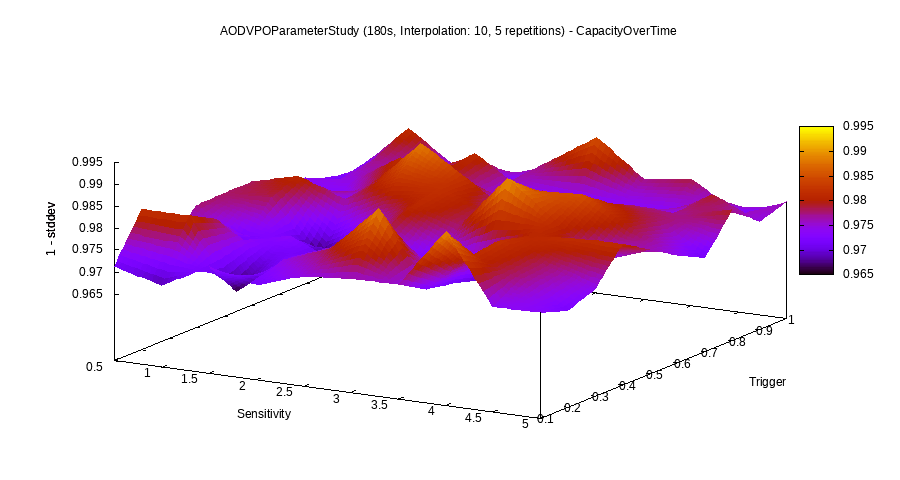
\includegraphics[scale=0.45]{bilder/o31.png} \\
\captionof{figure}{3D Darstellung Ladezustand ParameterStudy bei AODV, 180 Sekunden}
\end{center}

\begin{center}
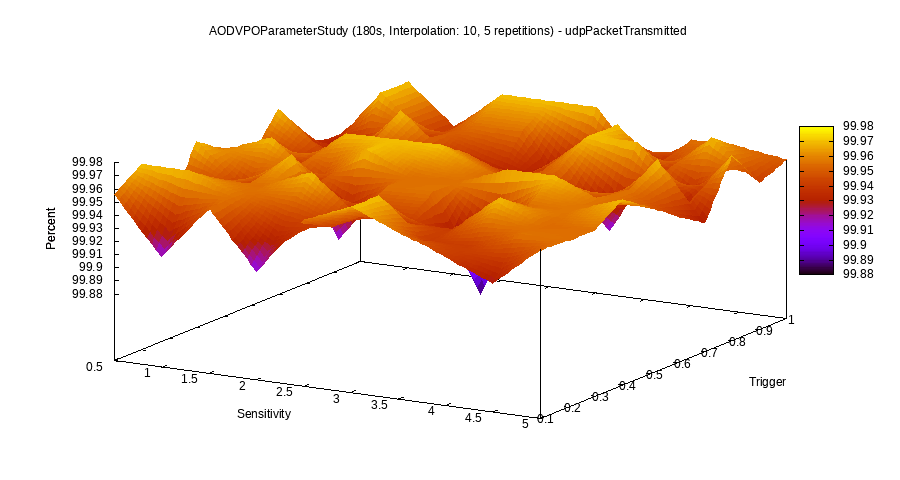
\includegraphics[scale=0.45]{bilder/o32.png} \\
\captionof{figure}{3D Darstellung PacketLoss ParameterStudy bei AODV, 180 Sekunden}
\end{center}

\newpage

\begin{center}
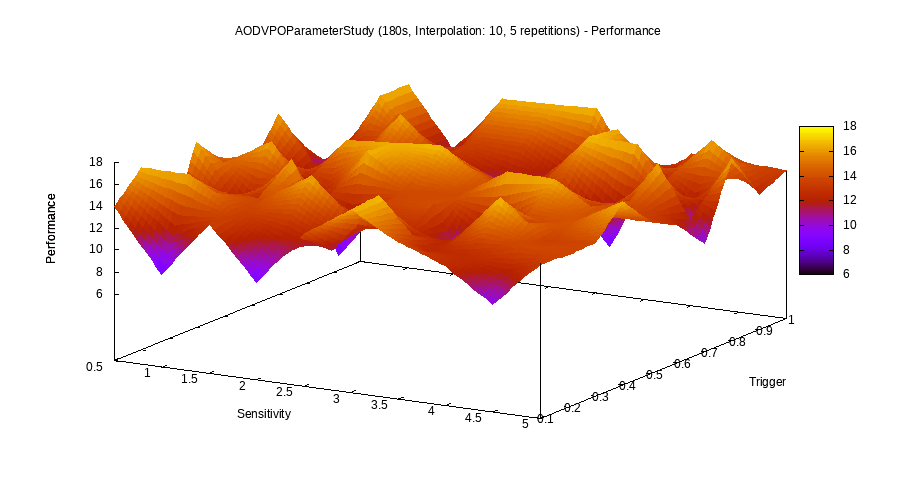
\includegraphics[scale=0.45]{bilder/o33.png} \\
\captionof{figure}{3D Darstellung Performance ParameterStudy bei AODV, 180 Sekunden}
\end{center}

\begin{center}
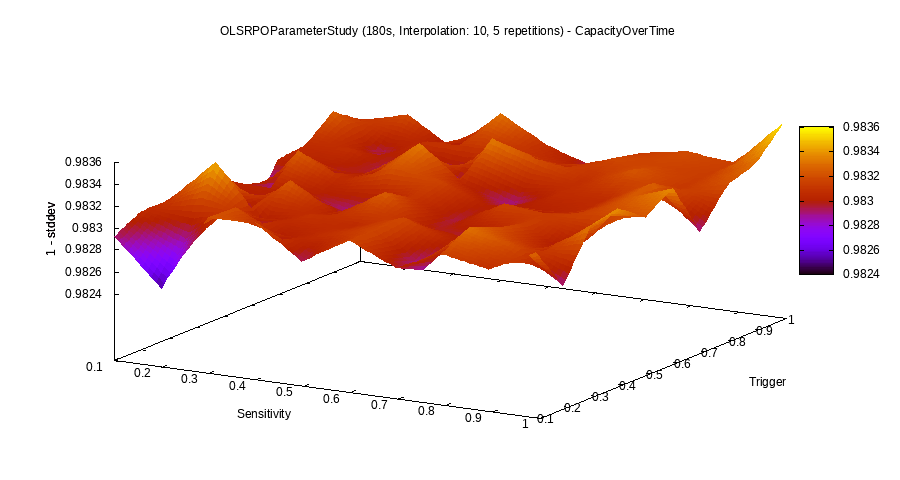
\includegraphics[scale=0.45]{bilder/o34.png} \\
\captionof{figure}{3D Darstellung Ladezustand ParameterStudy bei OLSR, 180 Sekunden}
\end{center}

\begin{center}
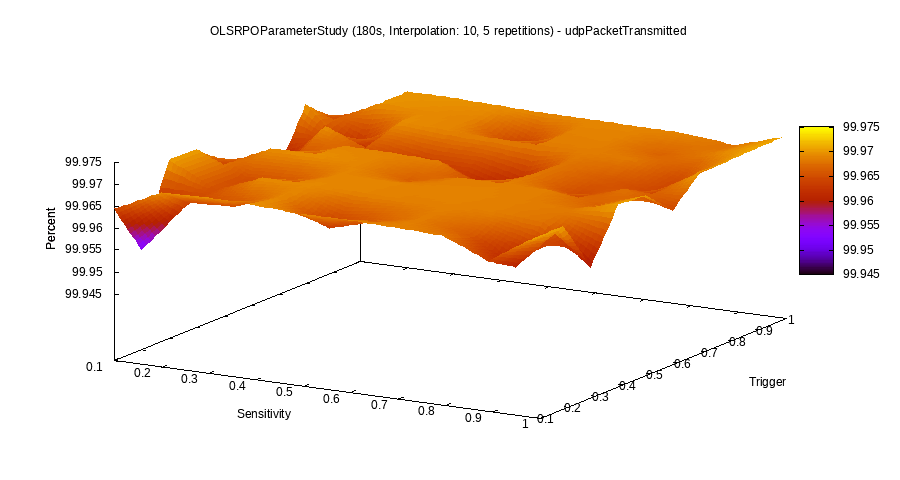
\includegraphics[scale=0.45]{bilder/o35.png} \\
\captionof{figure}{3D Darstellung PacketLoss ParameterStudy bei OLSR, 180 Sekunden}
\end{center}

\newpage

\begin{center}
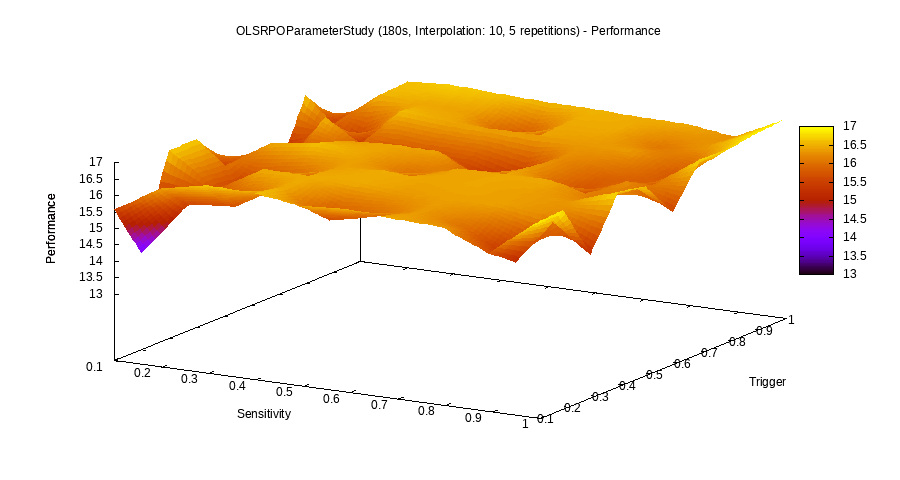
\includegraphics[scale=0.45]{bilder/o36.png} \\
\captionof{figure}{3D Darstellung Performance ParameterStudy bei OLSR, 180 Sekunden}
\end{center}
